% chapter4_system_design.tex
% Automated Diagram Digitization - System Design Chapter

\chapter{System Design}
\label{ch:systemdesign}

\justifying
This chapter presents the comprehensive system design of the Automated Diagram Digitization platform, detailing the architectural decisions, data flow, database schema, API design, and module specifications. The system design follows industry best practices for web applications, ensuring scalability, maintainability, security, and seamless integration between the frontend editor, backend services, and AI processing engine.

% =============================================================================
% 4.1 SYSTEM ARCHITECTURE OVERVIEW
% =============================================================================

\section{System Architecture Overview}
\label{sec:architecture}

\justifying
The Automated Diagram Digitization platform is built on a robust three-tier architecture ensuring scalability, maintainability, and security while providing seamless integration between the React frontend, FastAPI backend, and PostgreSQL database. This architectural model separates the system into three logical layers: the presentation layer responsible for user interaction, the application layer that implements the business logic and AI processing, and the data layer that manages persistent storage.

Such separation of concerns allows each tier to operate independently while communicating through well-defined interfaces. This improves maintainability because modifications in one layer do not directly affect the others. It also enables future scalability, allowing the frontend, backend, and database components to be deployed or upgraded independently based on system demand. The three-tier architecture is shown in below figure. \textit{Refer Figure~\ref{fig:ch4-architecture}: Three-tier system architecture}.

\begin{figure}[htbp]
    \centering
    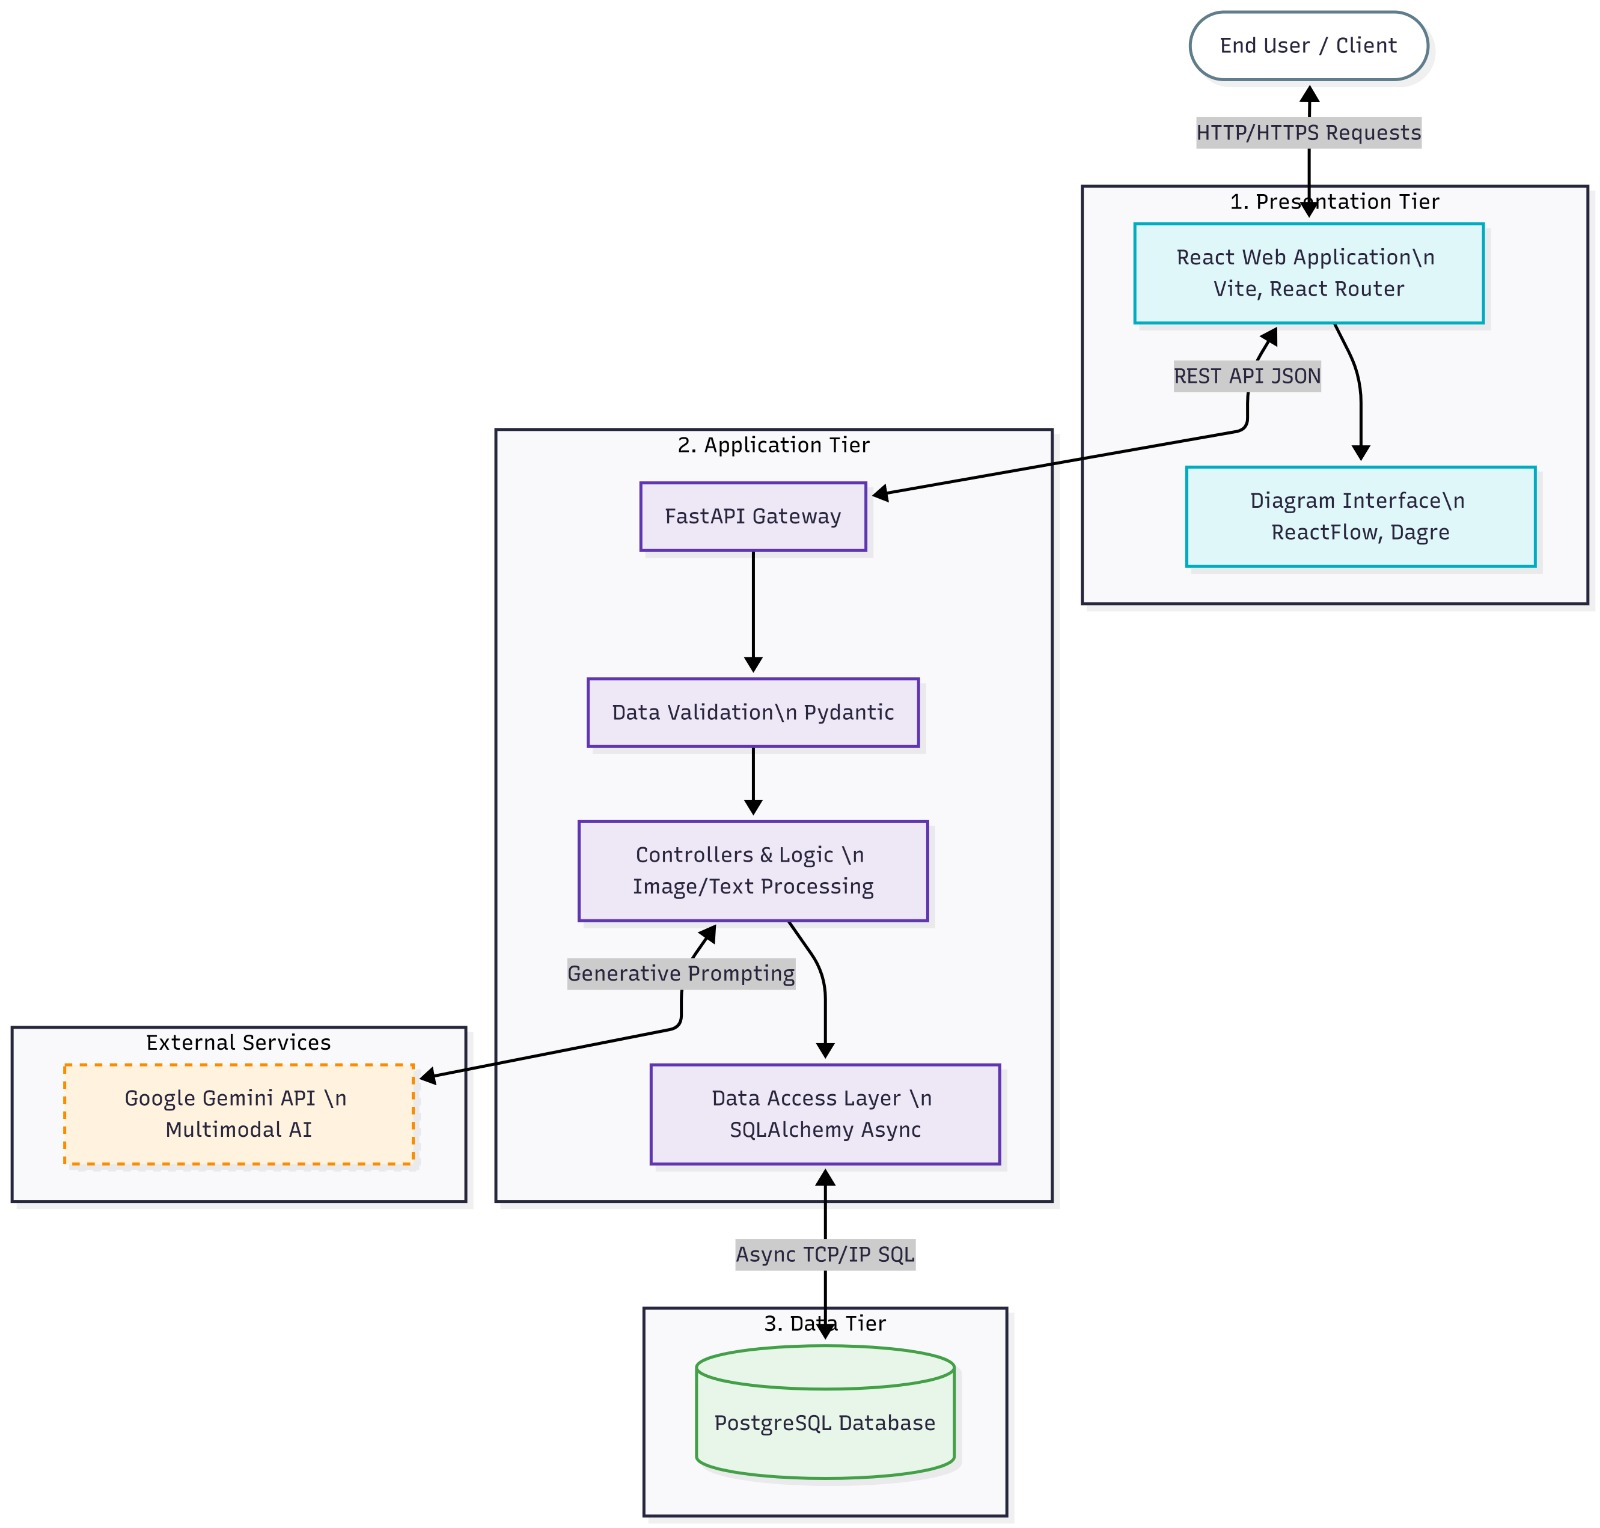
\includegraphics[width=\textwidth]{image/flow.jpg}
    \caption{Three-Tier System Architecture}
    \label{fig:ch4-architecture}
\end{figure}

\subsection{Presentation Layer (Client Tier)}

\justifying
The presentation layer serves as the user interface through which all users interact with the platform. It utilizes React~19 with Vite for fast development and optimal performance, React Flow for interactive diagram rendering, and Vanilla CSS for responsive, modern design.~\cite{react,vite,reactflow} Key advantages include component-based architecture for reusability, fast refresh during development, and a consistent experience across all devices and screen sizes.

\justifying
The interface is organized into two main sections: the input page with three tabs for image upload, text prompt, and JSON import; and the flowchart editor with a draggable shape sidebar, canvas area with background grid, and toolbar with undo/redo, auto-layout, export, and theme toggle controls. This structured interface design allows users to move smoothly between diagram input and editing stages without confusion. The tab-based input system ensures that multiple methods of diagram generation remain easily accessible, while the editor environment provides tools for refining and customizing the generated flowcharts. By combining these elements within a single interface, the platform offers a consistent workflow from diagram creation to final export.

\subsection{Application Layer (Business Tier)}

\justifying
The application layer implements all business logic, validation, workflow orchestration, and AI integration using FastAPI with Python. Key components include RESTful API endpoints for image analysis and text-to-flowchart generation, integration with Google Gemini AI using custom prompts, request validation using Pydantic models, centralized error handling with regex fallback for malformed responses, and asynchronous database operations using SQLAlchemy.

This layer acts as the central processing unit of the system, coordinating communication between the frontend interface, the AI processing service, and the database. By handling request validation, error handling, and response formatting in a centralized manner, the backend ensures consistent system behavior and simplifies debugging and maintenance tasks.

\subsection{Data Layer (Database Tier)}

\justifying
The data layer manages all persistent storage using PostgreSQL with JSONB support for flexible schema storage. Key features include UUID v4 primary keys for distributed generation without coordination, JSONB columns for storing complete React Flow state (nodes and edges), timestamp tracking with timezone support for \texttt{created\_at} and \texttt{updated\_at} fields, foreign key constraints where applicable, and connection pooling for optimal performance.

The database layer also supports efficient querying and reliable storage of flowchart data even as the number of diagrams grows over time. PostgreSQL's support for JSONB enables the system to store complex node and edge structures without requiring rigid relational schemas for every property. This flexibility allows the platform to support future enhancements such as additional node types, styling options, or metadata fields without requiring major database redesign.


% =============================================================================
% 4.2 DATA FLOW DIAGRAMS
% =============================================================================

\section{Data Flow Diagrams}
\label{sec:dfd}

\justifying
Data Flow Diagrams (DFDs) provide a graphical representation of how information moves through the Automated Diagram Digitization platform. They illustrate the sequence of data transformations that occur when users interact with the system, from initial input to final diagram output. By visualizing the movement of data between different system components, DFDs help clarify how the frontend interface, backend services, AI processing engine, and database interact during each workflow.

\subsection{Image Upload and Analysis Flow}

\justifying
The image analysis process enables users to upload flowchart images for automatic digitization. The workflow proceeds as follows: the user selects an image file via drag-drop or file picker, the frontend validates file type and size, the image is sent to the backend via multipart/form-data, the backend processes the image using Pillow (resizing to thumbnail), the image is sent to Gemini AI with the system prompt, the AI returns JSON with nodes and edges, the backend parses the response and ensures edge IDs exist, and the frontend renders the flowchart in the editor. The user can then edit, save, or export the diagram. The complete data flow for this process is illustrated. \textit{Refer Figure~\ref{fig:chapter4-image-flow}: Image Upload and Analysis Data Flow Diagram}.

\begin{figure}[!htbp]
    \centering
    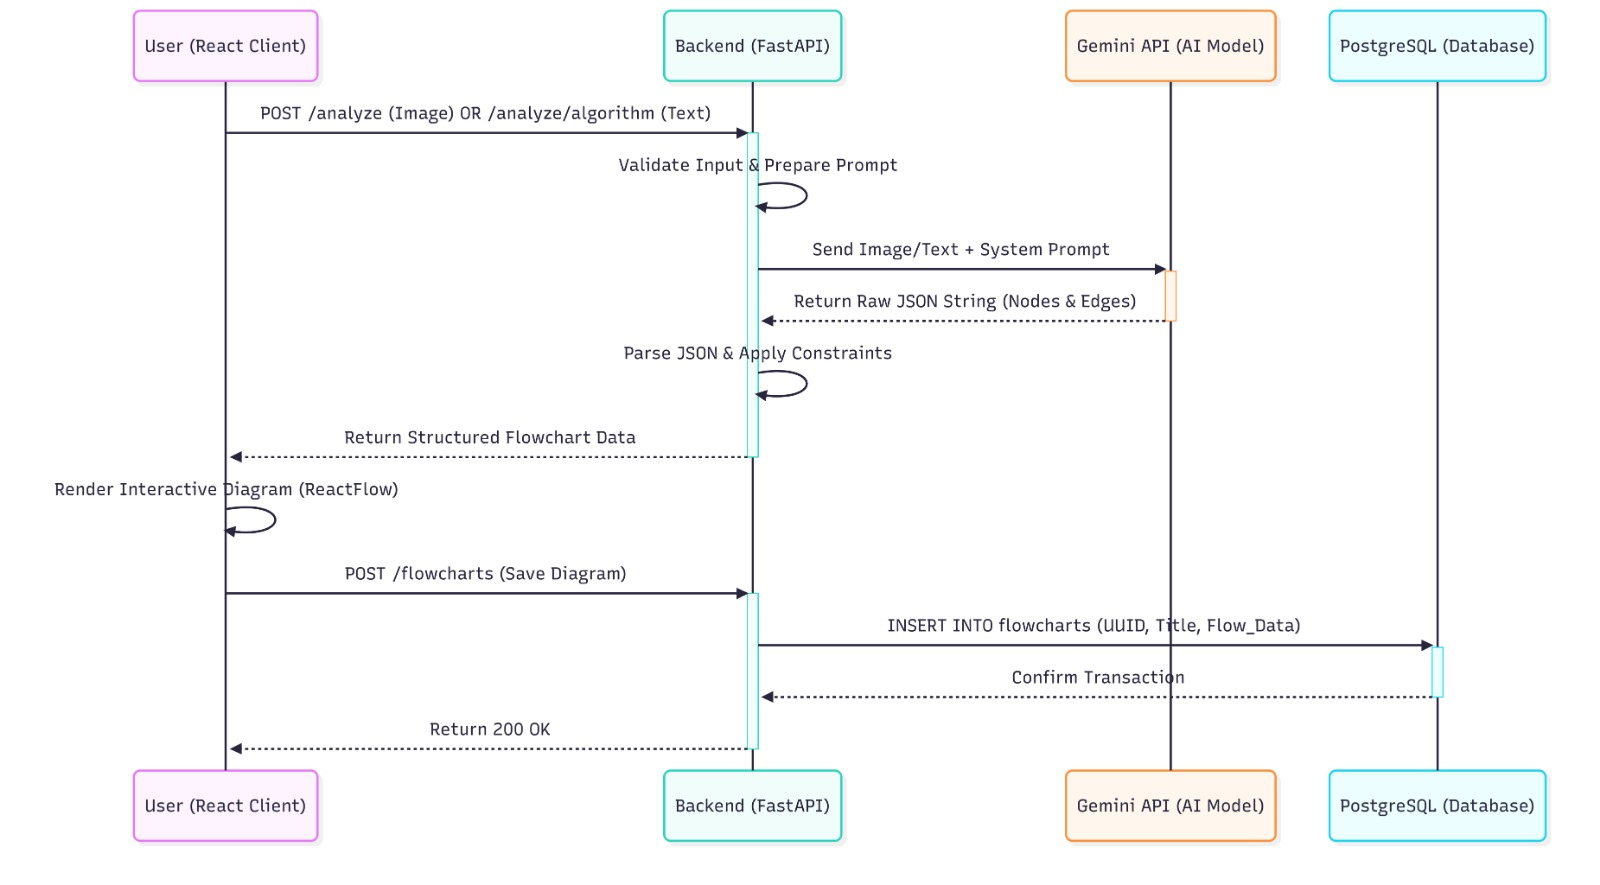
\includegraphics[width=0.95\textwidth]{image/df.jpg}
    \caption{Image Upload and Analysis Data Flow Diagram}
    \label{fig:chapter4-image-flow}
\end{figure}

\subsection{Text-to-Flowchart Generation Flow}

\justifying
The text-to-flowchart feature enables users to describe algorithms in natural language for automatic flowchart generation. The workflow proceeds as follows: the user enters a text description in the prompt textarea, the frontend sends the prompt to the backend via POST request, the backend combines the user prompt with the text-to-flowchart system prompt, the combined prompt is sent to Gemini AI, the AI returns JSON with nodes and edges (may include explanatory text), the backend extracts JSON using regex pattern matching, the parsed JSON is returned to the frontend, and the editor renders the generated flowchart. The user can then modify the generated diagram as needed.

\subsection{JSON Import and Export Flow}

\justifying
The JSON import/export functionality enables data portability and integration with other tools. For import: the user uploads a JSON file or pastes JSON into textarea, the frontend validates JSON format, the validated JSON is passed directly to the editor for rendering. For export: the user clicks the export button and selects format (JSON/PNG/SVG), for JSON export the current nodes and edges are serialized to JSON and downloaded as a file, for PNG export the canvas is captured using html-to-image and downloaded, for SVG export the React Flow SVG renderer generates vector graphics for download.

% =============================================================================
% 4.3 USE CASE DIAGRAM
% =============================================================================

\section{Use Case Diagram}
\label{sec:usecase}

\justifying
The Use Case Diagram (UCD) for the Automated Diagram Digitization platform describes the interactions between the system's single actor -- the user -- and the various functional capabilities the platform provides. The diagram captures the complete set of actions a user can perform within the system, from uploading a flowchart image to exporting the final diagram. The diagram illustrates the pivotal roles of the image analysis and text-to-flowchart generation modules, which serve as the primary entry points for system interaction. Users interact with the canvas interface to perform refined editing operations, such as modifying node labels, adjusting spatial configurations, and managing edge connections. Furthermore, the inclusion of an automated layout feature and persistent synchronization indicates a design focused on minimizing manual effort during diagram digitization. This comprehensive mapping of system functionality ensures that all intended user workflows are clearly defined and technically feasible within the platform's architectural boundaries. The use case diagram is presented below. \textit{Refer Figure~\ref{fig:use-case-diagram}: Use Case Diagram for Automated Diagram Digitization}.

\begin{figure}[!htbp]
    \centering
    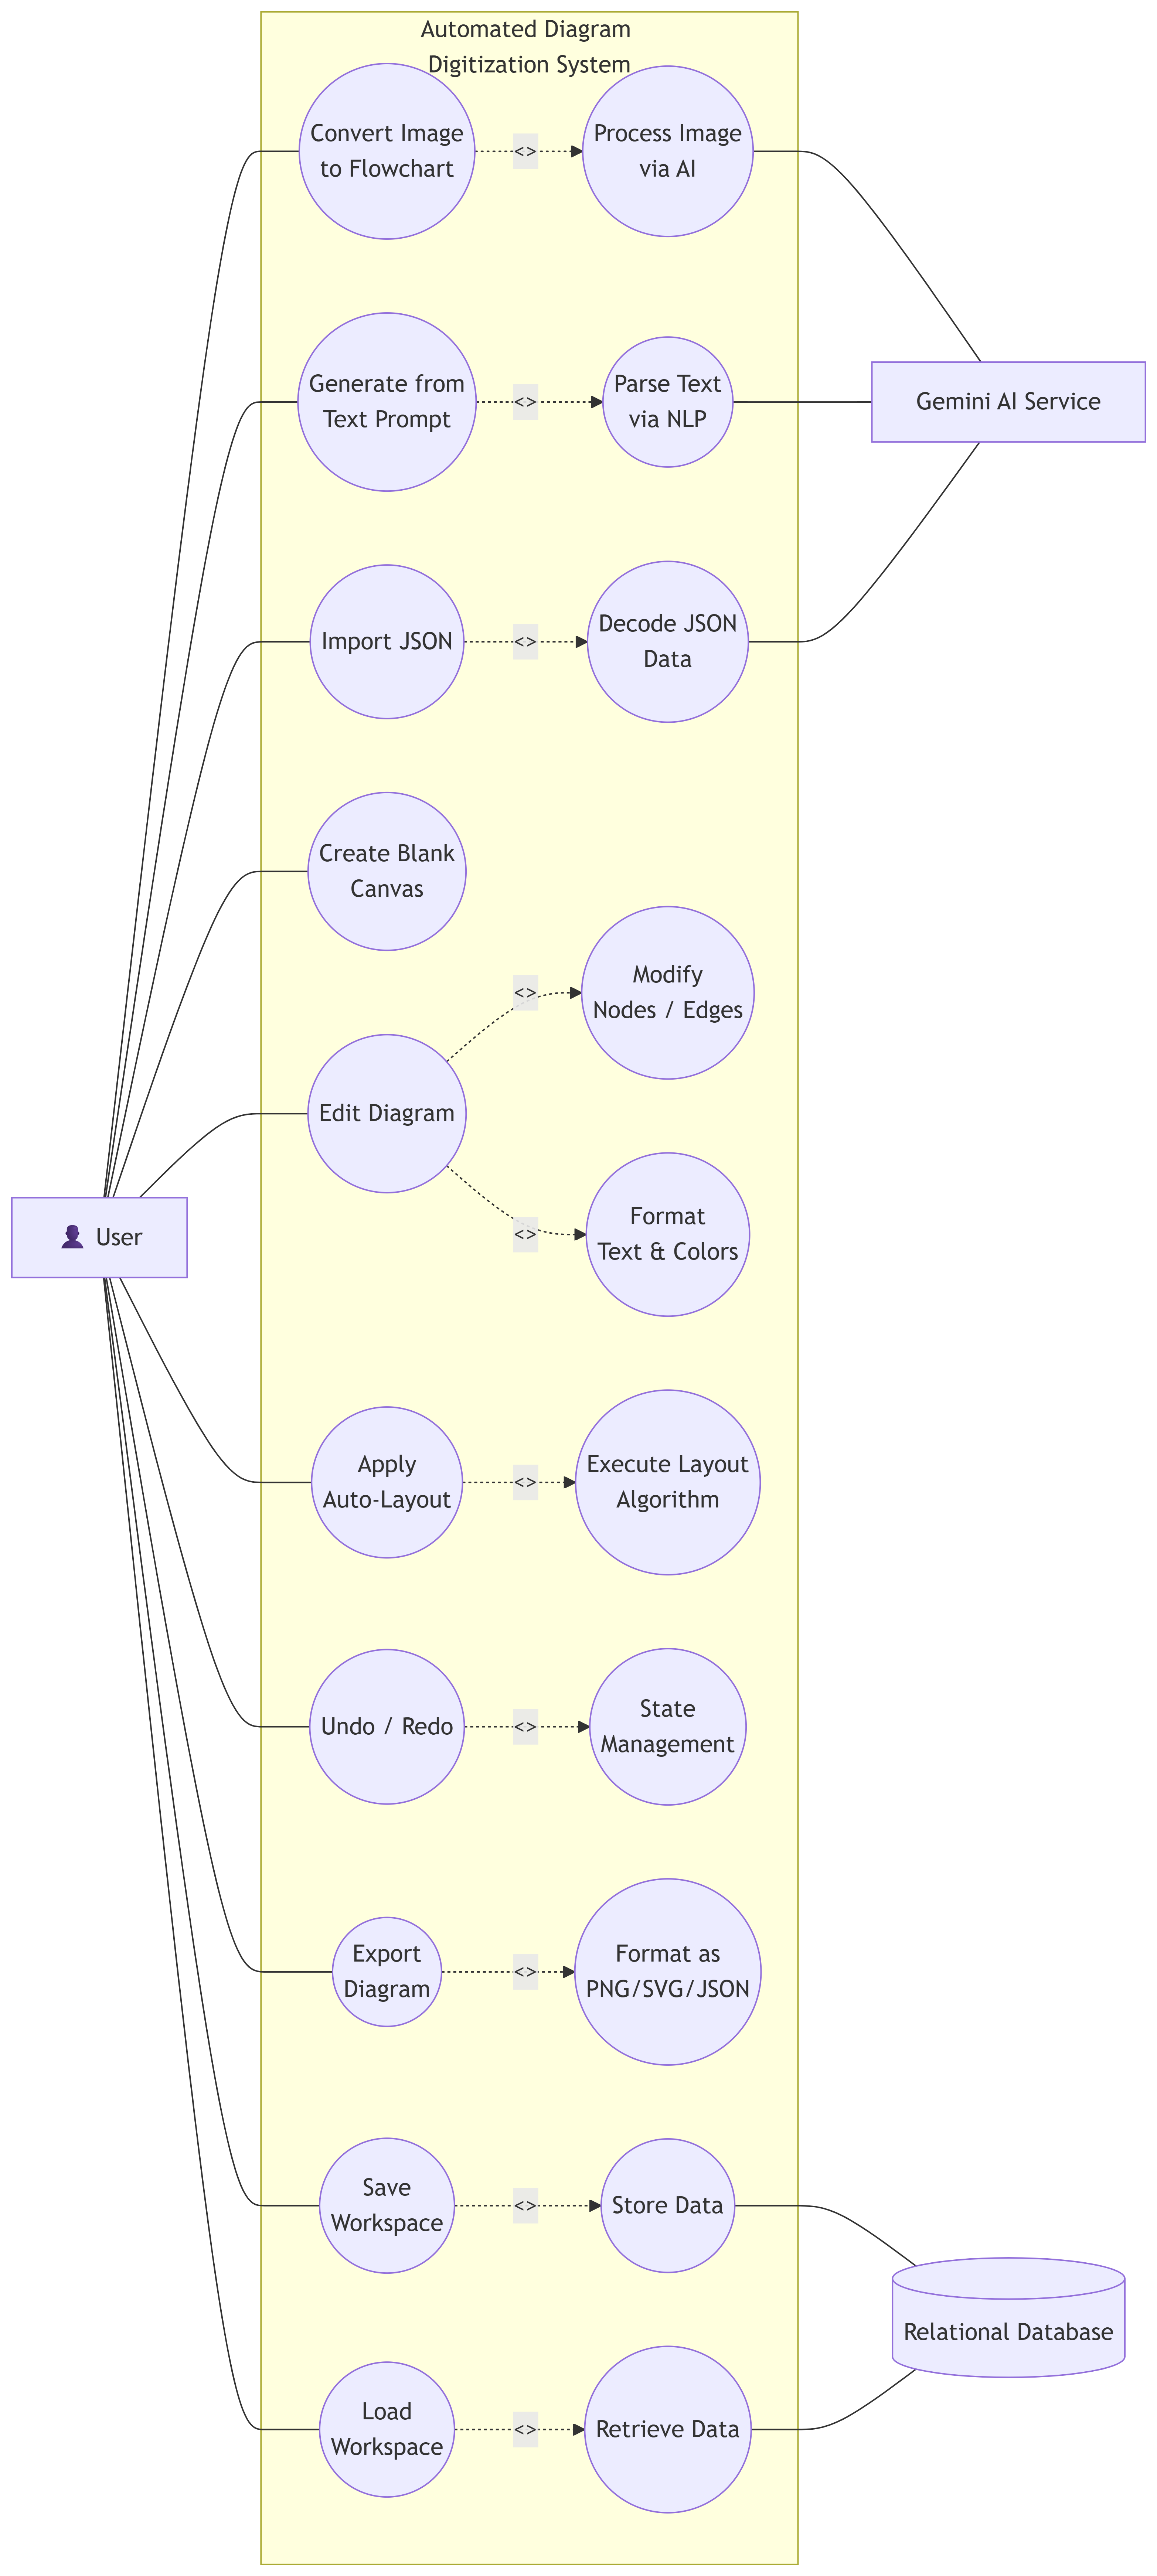
\includegraphics[width=\linewidth,height=0.95\textheight,keepaspectratio]{image/use-case-diagram.png}
    \caption{Use Case Diagram for Automated Diagram Digitization}
    \label{fig:use-case-diagram}
\end{figure}

% =============================================================================
% 4.4 DATABASE SCHEMA DESIGN
% =============================================================================

\section{Database Schema Design (PostgreSQL)}
\label{sec:dbschema}

\justifying
The Automated Diagram Digitization platform utilizes PostgreSQL with JSONB support, providing reliable data persistence, ACID compliance, and flexible schema for storing complex flowchart data. The schema uses UUID primary keys, timestamp tracking, and JSONB columns for flow data storage. The database schema is represented as a summary table; refer Table~\ref{tab:db_schema}: Database Schema Summary, and the entity-relationship diagram is illustrated in \textit{Refer Figure~\ref{tab:db_schema}: Database Schema Summary}.

\begin{table}[!htbp]
    \centering
    \renewcommand{\arraystretch}{1.3}
    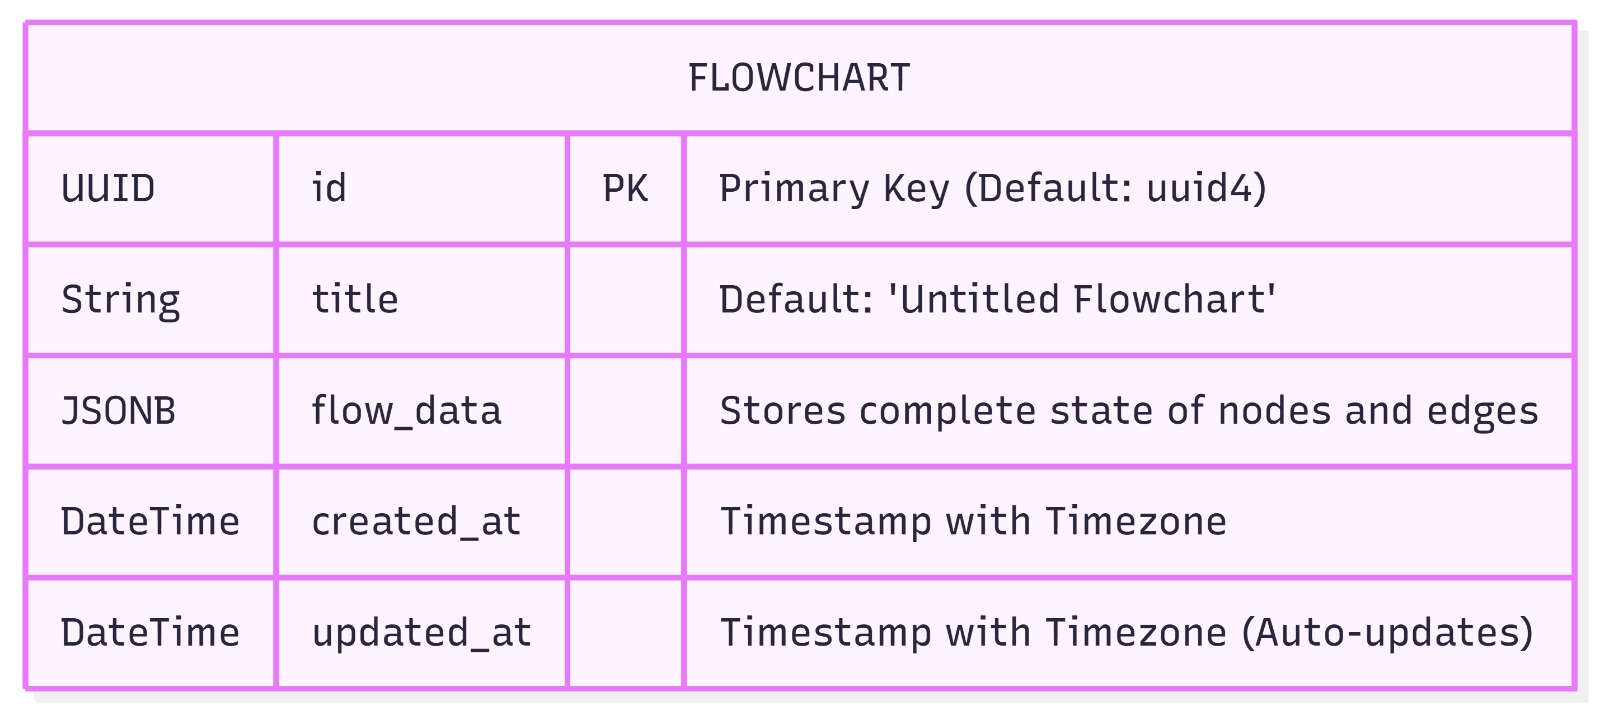
\includegraphics[width=0.8\textwidth,height=0.8\textheight,keepaspectratio]{image/arcch.jpg}
    \caption{Database Schema Summary}
    \label{tab:db_schema}
\end{table}

\justifying
The Entity-Relationship diagram above illustrates the database structure. At the center is the \texttt{flowcharts} table, which stores all flowchart data. Each flowchart has a unique UUID identifier, a title string, a JSONB column containing the complete React Flow state (nodes and edges), and timestamp columns for creation and last update tracking.
The JSONB column provides flexibility to store varying node and edge structures without requiring schema changes. Each node object contains id, type, position coordinates, data (including label), width, height, and optional styling properties. Each edge object contains id, source, target, optional label, type (smoothstep/straight), markerEnd for arrows, and optional styling properties. The schema follows best practices for web applications, uses \texttt{created\_at} and \texttt{updated\_at} timestamps with timezone support for audit compliance and uses UUID primary keys.

\justifying
All timestamp columns use \texttt{TIMESTAMPTZ} rather than a timezone-naive type, storing values in UTC and allowing the application layer to convert to the user's local timezone at render time. This is particularly important for a platform that may be deployed across different geographical regions. Consistent UTC storage eliminates ambiguity in timestamp comparisons.
The schema is managed through SQLAlchemy's declarative base, with tables automatically generated during application startup using the \texttt{Base.metadata.create\_all} method within the FastAPI lifespan context. This approach ensures that the database structure remains synchronized with the backend models without requiring manual SQL execution or external migration dependencies for the prototype deployment.


\subsection{Sample flow\_data JSON Structure}

\justifying
The \texttt{flow\_data} column stores the serialized state of the React Flow canvas, encompassing all structural and visual information of the diagram in a single JSON object. The sample below illustrates how nodes and edges are represented, including their unique identifiers, coordinate positions, and specific styling attributes required for consistent rendering. \textit{Refer Listing~\ref{lst:flowdata}: Sample flow\_data JSON Structure.}

\begin{lstlisting}[
    caption={Sample flow\_data JSON Structure},
    label={lst:flowdata},
    breaklines=true,
    columns=flexible,
    float=!htbp,
    basicstyle=\ttfamily\scriptsize]
{
  "nodes": [
    {
      "id": "node_123",
      "type": "process",
      "position": { "x": 100, "y": 200 },
      "data": { "label": "Process Data" },
      "width": 150,
      "height": 80,
      "style": {
        "backgroundColor": "#ffffff",
        "color": "#000000",
        "fontSize": 12,
        "fontWeight": "normal",
        "fontStyle": "normal"
      }
    },
    {
      "id": "node_456",
      "type": "decision",
      "position": { "x": 300, "y": 200 },
      "data": { "label": "Is Valid?\nYes/No" },
      "width": 120,
      "height": 120
    }
  ],
  "edges": [
    {
      "id": "e1-2",
      "source": "node_123",
      "target": "node_456",
      "sourceHandle": "bottom",
      "targetHandle": "top",
      "label": "Yes",
      "type": "smoothstep",
      "markerEnd": { "type": "arrowclosed" },
      "style": { "stroke": "#000000" },
      "labelStyle": {
        "fill": "#000000",
        "fontWeight": 600
      },
      "labelBgStyle": {
        "fill": "#ffffff",
        "stroke": "#000000",
        "strokeWidth": 1,
        "rx": 4,
        "ry": 4
      }
    }
  ]
}
\end{lstlisting}

% =============================================================================
% 4.5 API DESIGN
% =============================================================================

\section{API Design (RESTful Endpoints)}
\label{sec:api-design}

\justifying
The Automated Diagram Digitization platform implements a comprehensive RESTful API following industry best practices, serving as the communication backbone between the React frontend and FastAPI backend.Endpoints are resource-oriented, use appropriate HTTP methods, and consistent JSON response formats. The API is organised into logical resource groups: image analysis, text-to-flowchart generation, and flowchart management (CRUD operations). Middleware for CORS handling, request validation, and error handling is applied consistently. Incoming payloads are validated for type correctness, required fields, and domain constraints before any business logic executes.

Error responses follow a consistent JSON structure containing detail message and appropriate HTTP status codes: \texttt{200} for successful retrieval, \texttt{201} for resource creation, \texttt{400} for validation failures, \texttt{404} when a requested resource does not exist, and \texttt{500} for internal server errors. \textit{Refer Table~\ref{tab:api-endpoints}: Core API Endpoints.}

\begin{table}[htbp]
    \footnotesize
    \centering
    \renewcommand{\arraystretch}{1.5}
    \begin{tabular}{|>{\raggedright\arraybackslash}p{1.5cm}|>{\raggedright\arraybackslash}p{3cm}|>{\raggedright\arraybackslash}p{4cm}|>{\raggedright\arraybackslash}p{3cm}|}
        \hline
        \textbf{Method} & \textbf{Endpoint}  & \textbf{Description} & \textbf{Request Body} \\
        \hline

        POST & /analyze/image & Upload flowchart image for AI analysis
        & multipart/form-data (image file) \\
        \hline

        POST & /analyze/algorithm & Generate flowchart from text description
        & \texttt{\{"prompt": "text"\}} \\
        \hline

        POST & /flowcharts & Create new flowchart in database
        & \texttt{\{"title": "...", "flow\_data": \{...\}\}} \\
        \hline

        GET & /flowcharts & Retrieve list of all saved flowcharts (returns id, title, created\_at, updated\_at for each)
        & -- \\
        \hline

        GET & /flowcharts/\{id\} & Retrieve flowchart by UUID
        & -- \\
        \hline

        PUT & /flowcharts/\{id\} & Update existing flowchart
        & JSON with partial updates \\
        \hline

        GET & / & Health check endpoint
        & -- \\
        \hline

    \end{tabular}
    \caption{Core API Endpoints}
    \label{tab:api-endpoints}
\end{table}

\justifying
The AI model returns node positions on a normalized 0--1000 coordinate scale, regardless of the original image resolution. This normalization maintains consistent spatial relationships between nodes across images of varying dimensions. On the React frontend, these normalized coordinates are used directly as React Flow canvas positions, since React Flow's coordinate system is unbounded and scales with the viewport. Users can pan and zoom the canvas freely, with React Flow's built-in viewport transformation handling the mapping from canvas coordinates to screen pixels.

\subsection{Sample Request - Image Analysis}

\justifying
The image analysis request is initiated when a user uploads a diagram through the web interface. The frontend packages the image file as a multipart/form-data payload, ensuring that large binaries are transmitted efficiently. This request is sent to the \texttt{/analyze/image} endpoint, where the application layer prepares the file for processing by the AI back-end. \textit{Refer Listing~\ref{lst:image-request}: Image Analysis API Request.}

\begin{lstlisting}[
    caption={Image Analysis API Request},
    label={lst:image-request},
    breaklines=true,
    columns=flexible,
    basicstyle=\small\ttfamily,
    float=!htbp]
POST /analyze/image HTTP/1.1
Host: localhost:8000
Content-Type: multipart/form-data; boundary=----WebKitFormBoundary

------WebKitFormBoundary
Content-Disposition: form-data; name="file"; filename="flowchart.png"
Content-Type: image/png

[image data]
------WebKitFormBoundary--
\end{lstlisting}

\subsection{Sample Response - Image Analysis}

\justifying
Upon successful analysis, the system returns a structured JSON object representing the digitized flowchart. This response contains specific arrays for nodes and edges, defining shapes, labels, and directional connections. This structured format allows the React Flow engine to instantly recreate the visual diagram on the user's canvas. \textit{Refer Listing~\ref{lst:image-response}: Image Analysis API Response.}

\begin{lstlisting}[
    caption={Image Analysis API Response},
    label={lst:image-response},
    breaklines=true,
    columns=flexible,
    basicstyle=\small\ttfamily,
    float=!htbp]
{
  "nodes": [
    {
      "id": "1",
      "type": "start",
      "position": { "x": 500, "y": 50 },
      "data": { "label": "Start" },
      "width": 90,
      "height": 40
    },
    {
      "id": "2",
      "type": "process",
      "position": { "x": 475, "y": 150 },
      "data": { "label": "Enter\nCredentials" },
      "width": 150,
      "height": 80
    }
  ],
  "edges": [
    {
      "id": "e1-2",
      "source": "1",
      "target": "2",
      "sourceHandle": "bottom",
      "targetHandle": "top",
      "type": "smoothstep",
      "markerEnd": { "type": "arrowclosed" }
    }
  ]
}
\end{lstlisting}

% =============================================================================
% 4.6 MODULE-WISE DETAILED DESIGN
% =============================================================================

\section{Module-wise Detailed Design}
\label{sec:modules}

\justifying
This section provides design specifications for each major module of the Automated Diagram Digitization platform, describing their internal components and interactions with other modules. The modular architecture enables each functional component of the system to operate independently while contributing to the overall workflow. By separating responsibilities across modules, the system becomes easier to maintain, extend, and debug. Each module focuses on a specific task such as handling user input, processing AI-based recognition, editing diagrams, exporting results, or managing persistent storage. This modular approach ensures that enhancements or modifications to one part of the system can be implemented without significantly affecting other components.

\subsection{Input Module}

\justifying
The input module serves as the primary entry point for all diagram data, supporting multiple ingestion channels including image uploads, natural language prompts, and JSON imports. It performs essential data validation and pre-processing to ensure that incoming information is correctly formatted for the AI recognition and editing layers. The input module consists of several integrated components that work together to simplify the diagram ingestion process. The image upload component provides a drag-and-drop zone with a file picker fallback, ensuring compatibility with PNG, JPG, and WebP formats while performing file type and size validation. For users who prefer textual input, the text prompt component offers a multi-line textarea with a character count and example algorithm descriptions. JSON data portability is enabled through a dedicated import component that supports both file uploads and direct pasting with real-time syntax validation. All these ingestion methods are unified within a responsive tabbed navigation interface that allows users to switch between modes seamlessly while maintaining an active state for the current operation.

\subsection{AI Processing Module}

\justifying
The AI processing module coordinates the interaction between the system and the Google Gemini API, acting as the bridge for flowchart recognition. It manages the lifecycle of AI requests, from initial prompt construction and image optimization to the final parsing of unstructured AI output into system-compatible objects.

The AI processing module is composed of dedicated components that manage the end-to-end communication with external services. The Gemini API client handles secure authentication using environment-based keys and manages the transmission of multimodal requests. Image optimization is performed by an internal processor using the Pillow library, which resizes images to a maximum of 1024x1024 pixels to ensure rapid processing without sacrificing recognition accuracy. A centralized prompt manager organizes the complex system instructions for both image analysis and text-to-flowchart generation, ensuring that user inputs are contextualized correctly. Once the AI returns a result, the response parser utilizes regular expressions to extract structured JSON data, handles malformed outputs, and ensures that all nodes and edges conform to the system’s internal schema. Finally, a dedicated error handler catches API exceptions and provides user-friendly notifications and fallback mechanisms when necessary.

\subsection{Editor Module}

\justifying
The editor module provides a high-performance interactive workspace where users can refine and personalize their digitized diagrams. Built on React Flow, it handles complex state management and real-time canvas updates, ensuring a seamless experience when dragging, resizing, or styling flowchart components.

The editor module provides a comprehensive suite of tools for refined diagram manipulation. The core React Flow canvas renders the diagram with a background grid and handles zooming, panning, and element selection. Shapes are introduced via a sidebar palette that supports HTML5 drag-and-drop actions for different flowchart symbols. Each shape is rendered using custom node components that support both standardized rendering and individual styling. Node resizing is managed by a dedicated resizer component that maintains minimum dimensions while ensuring text readability. For edge connectivity, an inline label editor appears on double-click, allowing for rapid categorization of flow paths. The module also includes a sophisticated undo and redo system based on state snapshots, ensuring that every user action can be reverted or restored. Diagram organization is further enhanced by an auto-layout engine that applies a custom column snapping algorithm for perfect vertical alignment. Users can personalize their diagrams through integrated styling controls, which provide access to color pickers and advanced text formatting options.

\subsection{Export Module}

\justifying
The export module facilitates the final stage of the diagram workflow by converting the internal JSON state into shareable and portable formats. It supports high-resolution image generation for documentation as well as structured data exports, allowing users to move their work between different platforms or archival systems. Components include a PNG exporter that uses the html-to-image library to generate high-resolution image files, and an SVG exporter that leverages React Flow’s vector rendering for infinite scalability. Additionally, a JSON exporter serializes the current canvas state into a structured and indented JSON file for data portability. These features are consolidated within a centralized export menu that provides visual feedback and icons for each supported format.

\subsection{Storage Module}

\justifying
The storage module is responsible for the persistent management of flowchart data, ensuring that user work is saved reliably and can be retrieved across sessions. It leverages SQLAlchemy to provide an asynchronous abstraction over the PostgreSQL databas, utilizing the JSONB data type to store complex diagram states with high performance and flexibility.~\cite{sqlalchemy,postgresql}

The module’s core components include an asynchronous database client that utilizes SQLAlchemy’s engine with connection pooling for optimized performance. It supports a full suite of create, read, and update operations, enabling the system to save new diagrams with UUID identifiers, retrieve existing flowcharts with their full JSONB state, and apply partial updates to titles or flow data while automatically maintaining audit timestamps.

\subsection{Theme Module}

\justifying
The theme module delivers a customized visual experience by managing the application's appearance settings. It coordinates the synchronization of dark and light mode preferences using React Context and CSS variables, ensuring that theme changes are applied instantly throughout the entire component hierarchy without requiring a full page reload. Theme management is enabled through a dedicated React context that provides global theme state and toggle functions to the entire application. The interface includes a theme toggle button with adaptive icons that triggers these changes and persists the user’s preference in local storage. Dynamic styling is achieved through root-level CSS variables that are updated instantly on theme change, ensuring that node backgrounds, borders, and canvas colors adapt to the selected mode while maintaining consistent persistence across sessions.

% =============================================================================
% 4.7 AI PROMPT DESIGN
% =============================================================================

\section{AI Prompt Design}
\label{sec:prompt-design}

\justifying
Prompt design is a critical component of the system's intelligence, where natural language instructions are meticulously structured to guide the Google Gemini model. These prompts define the rules for shape recognition, coordinate systems, and JSON formatting, ensuring that the AI provides deterministic and physically accurate flowchart representations.~\cite{gemini}

\subsection{Image Analysis System Prompt}

\justifying
The image analysis system prompt is carefully engineered to instruct Gemini AI to act as an Optical Graph Recognition engine. It defines strict rules for identifying node shapes, extracting positional coordinates, determining edge connections, and returning the result as raw structured JSON compatible with React Flow. By specifying a normalized coordinate system (0--1000), the prompt ensures that the spatial relationships between nodes are preserved regardless of the original image's aspect ratio. It also enforces a strict mapping of visual shapes to specific system-defined node types, such as \texttt{process} for rectangles and \texttt{decision} for diamonds, to maintain graphical consistency. Additionally, the prompt explicitly forbids the inclusion of conversational preamble or markdown formatting, which significantly reduces parsing overhead on the application server. This deterministic approach allows the backend to reliably transform raw visual data into a serialized state that can be immediately rendered by the React Flow engine. \textit{Refer Listing~\ref{lst:image-prompt}: Image Analysis System Prompt.}~\cite{reactflow}

\begin{lstlisting}[language=Python,
    caption={Image Analysis System Prompt},
    label={lst:image-prompt},
    breaklines=true,
    columns=flexible,
    keepspaces=true,
    basicstyle=\scriptsize\ttfamily,
    float=htbp]
SYSTEM_PROMPT = """
You are an expert Optical Graph Recognition engine.Analyze the provided flowchart image and extract its structure into a JSON format compatible with React Flow.

Follow these strict rules:

1. Nodes:
- Identify shapes and map to these EXACT types:
  - rectangle -> type: "process"
  - diamond -> type: "decision"
  - oval/circle -> type: "start"
  - parallelogram -> type: "io"
- Dimensions: Calculate the actual width and height of each shape based on its bounding box in the image (relative to a 1000x1000 canvas).
- Extract text into data.label (use \\n for line breaks).
- Estimate coordinates on a 0-1000 scale.

Output each node as:
{
  "id": "1",
  "type": "process",
  "position": { "x": 500, "y": 100 },
  "width": 150,
  "height": 80,
  "data": { "label": "Text Here" }
}

2. Edges:
- 'type': "smoothstep"
- 'markerEnd': { "type": "arrowclosed" }
- 'sourceHandle' and 'targetHandle': Use "top", "bottom", "left", or "right" based on where the arrow physically enters/exits the shape in the image.
  - Default exit: "bottom"
  - Default entry: "top"
  - Decision side exits: "left" or "right"
  - Back-loops: Use "left" or "right" for targetHandle to avoid line overlapping.

Output each edge as:
{
  "id": "e1-2",
  "source": "1",
  ...
  "type": "smoothstep",
  "markerEnd": { "type": "arrowclosed" }
}

3. Output format:
- Return ONLY raw JSON. No markdown, no backticks, no preamble.
- Structure: {"nodes": [...], "edges": [...]}
"""
\end{lstlisting}

\subsection{Text-to-Flowchart System Prompt}

\justifying
The text-to-flowchart system prompt guides Gemini AI in converting natural language process descriptions into structured React Flow JSON. It specifies the allowed node types, layout sizing rules, edge connection conventions, and label formatting requirements to ensure consistent and well-structured flowchart output. Furthermore, the prompt identifies specific semantic markers within the algorithm description to determine decision branches and iterative loops, ensuring that complex logical structures are translated with high fidelity. This instructional framework minimizes the risk of structural ambiguity, allowing the AI to generate a functional diagram that accurately reflects the user's original algorithmic intent. \textit{Refer Listing~\ref{lst:text-prompt}: Text-to-Flowchart System Prompt.}
\begin{lstlisting}[language=Python,
    caption={Text-to-Flowchart System Prompt},
    label={lst:text-prompt},
    breaklines=true,
    columns=flexible,
    keepspaces=true,
    basicstyle=\scriptsize\ttfamily,
    float=htbp]
TEXT_TO_FLOW_PROMPT = """
You are a React Flow architect. Convert the user's process description or algorithm into a structured JSON.
Output ONLY raw JSON.

1. Node Rules (Strict Boundaries):
- TYPES: You MUST use only: "start", "process", "decision", "io".
- ROOT-LEVEL DIMENSIONS: width and height MUST be at the root level of the node object.
- DYNAMIC SCALING RULE: 
    * If a label has many lines, you MUST increase width/height to maintain a 25px clear internal margin.
    * FOR 'decision' DIAMONDS: Because corners cut inward, the node size must be at least 2.5x the width of the longest text line. 
    * If text in a diamond is 5+ lines, the node size MUST be at least 200x200.
- FONT SIZE: Assume 12px font. 

2. Example Dynamic Structure:
{
  "id": "unique_id",
  "type": "decision",
  "position": {"x": x, "y": y},
  "data": {"label": "Is the current\\ntemperature...?"},
  "width": 220,  # AI scales this up from 120 to fit text
  "height": 220
}

3. Edge & Label Rules:
- Use "type": "smoothstep" and "markerEnd": {"type": "arrowclosed"}.
- Use "sourceHandle" and "targetHandle" (top, bottom, left, right) for clean connections.
- For decision branches (Yes/No), include these exact styling properties:
  "label": "Yes",
  "labelStyle": {"fill": "#000", "fontWeight": 700},
  "labelBgStyle": {"fill": "#fff", "fillOpacity": 0.9, "stroke": "#000", "strokeWidth": 1},
  "labelBgPadding": [8, 4],
  "labelBgBorderRadius": 4
  
4. Label & Text Rules (Rhombic Typesetting):
- IMPORTANT: Labels MUST stay within the diamond's safety zone.
- VISUAL SHAPING: For 'decision' nodes, format the text block like a rhombus:
    * The first line must be 1-2 short words; 
    * The middle lines must be the longest.
- LINE LENGTH: Middle lines can be up to 18-20 characters.
- VERTICAL ALIGNMENT: Use exactly 1 newline (\\n) between lines.
- DYNAMIC SCALING: If the text is long, you MUST increase 'width' and 'height' to at least 2.5x the longest line length.
"""
\end{lstlisting}


% =============================================================================
% 4.8 ALGORITHM DESIGN
% =============================================================================

\section{Algorithm Design}
\label{sec:algorithm}

\justifying
The Automated Diagram Digitization platform incorporates several internal algorithms to support diagram generation, layout organization, and editing functionality. These algorithms are responsible for maintaining structural consistency within generated diagrams and ensuring that editing operations remain efficient and reliable. Algorithmic design plays a critical role in transforming raw AI-generated data into visually organized flowcharts. By applying structured layout techniques and maintaining editing history through snapshot mechanisms, the system provides users with both automated organization and flexible manual control during diagram creation.

\subsection{Column Snapping Auto-Layout Algorithm}

\justifying
The auto-layout feature utilizes a custom \textbf{Column Snapping (1D Clustering)} algorithm to organize nodes into a visually structured and aligned format. When diagrams are generated automatically or manually edited, physical overlaps and uneven vertical spacing can occur. This algorithm corrects these issues by detecting implicit vertical columns and snapping nodes to a common center line, ensuring a professional and structured appearance.

\justifying
The algorithm operates in four distinct phases: column detection, center alignment, width normalization, and edge type optimization. During column detection, the algorithm scans all nodes and groups them into vertical columns if their horizontal positions are within a specific 150px tolerance, sorting them by true center coordinates to ensure sequential clustering. In the center alignment phase, it calculates the average center-X coordinate for each group and snaps all nodes in that specific column to that exact center line, accounting for individual node widths to maintain visual balance. To ensure visual consistency, the width normalization phase calculates the maximum width for each node type and applies it globally across the flowchart, preventing varied sizes within the same category. Finally, in the edge type optimization phase, the engine determines the optimal edge style; if source and target nodes are aligned within a 50px threshold, the edge is switched to a straight type, otherwise, it uses a smoothstep style for a clean, forked appearance.
As a result, the flowchart becomes visually balanced and aligned, emphasizing logical progression and improving overall readability with minimal manual intervention.

\subsection{Undo and Redo Snapshot Algorithm}

\justifying
The platform includes an undo and redo mechanism that allows users to revert or restore modifications made while editing diagrams. This feature is implemented using a snapshot-based history management algorithm. Whenever a user performs an operation that modifies the diagram, such as adding a node, deleting an edge, moving an element, or changing text content, the system captures a snapshot representing the complete state of the diagram at that moment. Each snapshot contains the full set of nodes and edges currently present in the flowchart.

Snapshots are stored in a history structure consisting of two stacks referred to as the \textit{past} stack and the \textit{future} stack. The past stack records previous states of the diagram, while the future stack stores states that can be restored through redo operations. When a user performs an undo operation, the system retrieves the most recent snapshot from the past stack and restores the diagram to that earlier state. At the same time, the current state of the diagram is stored in the future stack, allowing it to be restored later if necessary.

If the user performs a redo operation, the system retrieves the next snapshot from the future stack and applies it to the diagram. The previously restored state is then returned to the past stack. This two-stack mechanism allows users to move backward and forward through their editing history without losing information. Keyboard shortcuts such as \texttt{Ctrl+Z} for undo and \texttt{Ctrl+Y} or \texttt{Ctrl+Shift+Z} for redo provide quick access to these operations, improving usability during diagram editing.

\justifying
Together, these algorithms ensure that diagrams remain organized and editable while providing users with flexible control over the editing process. The auto layout algorithm enhances visual clarity by maintaining alignment among nodes, while the snapshot-based history system provides reliable recovery from editing mistakes.


% =============================================================================
% 4.9 ERROR HANDLING DESIGN
% =============================================================================

\section{Error Handling Design}
\label{sec:error-handling}

\justifying
A resilient system requires careful planning for unexpected inputs and external service failures. The platform's error handling design uses a multi-layered approach to detect, log, and recover from issues occurring during AI processing, database interactions, or client-side operations, maintaining a stable experience for the end user.

\subsection{AI Response Error Handling}
\label{sec:ai-error}

\justifying
The backend implements several strategies to gracefully handle imperfect or malformed responses returned by the Gemini AI model. These mechanisms ensure the system can recover from common AI output issues without crashing or returning errors to the user.

The backend utilizes several integrated strategies to ensure robustness against imperfect AI responses. Malformed JSON blocks are identified and extracted from conversational text using regular expressions, while unescaped or unconventional characters within strings are handled by passing the raw response through a JSON parser with strict formatting disabled. Furthermore, the system validates that all required node and edge fields are present, providing logical defaults when necessary. To maintain connectivity data, any missing edge identifiers are automatically generated based on their source and target nodes, ensuring that the diagram remains structurally sound even if the AI provides incomplete metadata.

The primary mechanism for handling malformed AI responses is a regular expression extraction fallback. When the Gemini model returns a response containing explanatory text alongside the JSON structure, the backend applies the following pattern to isolate the JSON content. \textit{Refer Listing~\ref{lst:regex_fallback}: Regex JSON Extraction Fallback}.

\begin{lstlisting}[language=Python,
    label={lst:regex_fallback},
    caption={Regex JSON Extraction Fallback},
    breaklines=true,
    columns=flexible,
    float=htbp]
# 1. Clean response of any chatty AI text
text_response = response.text.strip()

# 2. Use regex to find the actual JSON block { ... }
match = re.search(r'(\{.*\})', text_response, re.DOTALL)

if match:
    json_str = match.group(1)
    try:
        # 3. USE strict=False to handle \n characters
        return json.loads(json_str, strict=False)
    except json.JSONDecodeError:
        # 4. Emergency cleaning for single quotes or unescaped newlines
        fixed_json = json_str.replace("'", '"').replace('\n', '\\n')
        return json.loads(fixed_json, strict=False)
\end{lstlisting}

The \texttt{re.DOTALL} flag allows the pattern to match across multiple lines, enabling the regex to capture deeply nested JSON objects spanning many response lines. The \texttt{strict=False} parameter in \texttt{json.loads()} handles responses containing unescaped newline characters within string values, which the Gemini model occasionally produces. Additionally, an emergency \texttt{replace} operation is performed to correct common syntax errors like single quotes used as delimiters or unescaped newlines before a final parsing attempt.

\subsection{API Error Handling}

\justifying
The API layer returns standardized HTTP error responses to clearly communicate the nature of any failure to the client. Each error code corresponds to a specific category of problem, making it straightforward for the frontend to respond appropriately.

Standardized HTTP status codes are used to communicate local and upstream errors transparently. A 400 Bad Request is returned for validation failures or missing parameters, while a 404 Not Found is issued if a requested flowchart ID does not exist in the database. For critical failures such as database disconnection or AI service unavailability, the system returns a 500 Internal Server Error along with detailed logging for administrative review.

\subsection{Frontend Error Handling}

\justifying
The frontend implements client-side validation and error display mechanisms to provide users with immediate and informative feedback when issues occur during file upload, JSON import, or API communication.

The frontend provides immediate feedback through a variety of validation and notification mechanisms. File upload errors related to type or size are caught before transmission, while JSON import errors provide descriptive messages that pinpoint exact syntax issues. Additionally, all API request failures are caught globally and displayed as transient toast notifications, often providing the user with an option to retry the operation.

% =============================================================================
% 4.10 PERFORMANCE OPTIMIZATION
% =============================================================================

\section{Performance Optimization}
\label{sec:performance}

\justifying
Providing a seamless and responsive user interface is essential for professional diagramming tools. The performance optimization strategy focuses on reducing latency and minimizing resource consumption across all system layers, from efficient binary transmission on the backend to optimized rendering cycles in the interactive editor.

\subsection{Backend Optimization}

\justifying
Backend performance is optimized through techniques that minimize processing time and maximize throughput. By implementing advanced image pre-processing before API calls and leveraging asynchronous database operations, the system can handle concurrent requests while maintaining low response times for data-intensive tasks.

To maximize performance, the backend incorporates image pre-processing and efficient data management techniques. Images are resized to a maximum of 1024 pixels before being sent to the AI, which significantly reduces network latency and processing time. Database connectivity is managed through SQLAlchemy connection pooling with a configurable size to minimize initialization overhead, while asynchronous endpoints allow for high concurrency during AI and storage operations. Furthermore, the system includes GIN indexes on JSONB columns to support future high-performance querying requirements.

\subsection{Frontend Optimization}

\justifying
The frontend utilizes modern React optimization patterns to ensure that the interactive canvas remains smooth even with hundreds of nodes. Techniques such as component memoization, virtualization of large datasets, and code-splitting are employed to minimize the main-thread workload and reduce the initial application bundle size.

Frontend performance is maintained through strategic rendering and loading patterns. Large diagrams leverage React Flow’s virtualization to only render visible elements, while memoization and specialized hooks are used to limit unnecessary component updates. Heavy operations like auto-saving and layout adjustments are debounced to ensure the main thread remains responsive. Additionally, the application bundle is kept small through code-splitting and lazy loading, while global visual changes like theme switching are executed instantly using CSS variables.

\subsection{AI Optimization}

\justifying
AI interactions are optimized to balance recognition accuracy with operational speed. By fine-tuning prompt lengths, using deterministic parameters (temperature=0), and pre-scaling images to optimal resolutions, the system reduces API costs and provides faster feedback loops during diagram digitization and generation.

AI-related optimizations balance recognition quality with operational efficiency. Prompt engineering techniques such as parameter tuning and specific MIME type declarations ensure consistent, deterministic outputs. Pre-scaling images to optimal resolutions further reduces API latency and costs, while the use of multi-stage Docker builds ensures that the entire orchestration of services remains performant and resource-efficient.

% =============================================================================
% 4.12 CONTAINERIZATION AND DEPLOYMENT
% =============================================================================

\section{Containerization and Deployment}
\label{sec:deployment}

\justifying
The Automated Diagram Digitization platform adopts a distributed cloud-based deployment architecture to ensure scalability, flexibility, and ease of maintenance. Instead of relying on a unified container orchestration approach in production, the system components are deployed independently across specialized platforms optimized for their respective roles.

\justifying
The frontend, developed using React, is deployed on Vercel, which provides optimized static hosting, automatic scaling, and global content delivery. The backend, built with FastAPI, is deployed on Render, where it runs as a web service with environment-based configuration and managed deployment pipelines. The database layer is provisioned using a PostgreSQL service, ensuring persistent and reliable data storage with secure connection management.

This separation of concerns allows each component to scale independently and leverage platform-specific optimizations. While Docker-based containerization may be used during local development to ensure environment consistency and simplify setup, the production deployment follows a cloud-native model that enhances reliability, performance, and maintainability.

% =============================================================================
% 4.11 CONCLUSION
% =============================================================================

\section{Conclusion}
\label{sec:ch4-conclusion}

\justifying
This chapter has presented the complete system design of the Automated Diagram Digitization platform, spanning the three-tier architecture, data flow diagrams, database schema, API design, module specifications, AI prompt design, algorithms, error handling, and performance optimization strategies. The design decisions reflect consistent priorities: accurate AI-powered recognition, intuitive user experience, robust error handling, and scalable architecture.

\justifying
The layered separation between presentation, business logic, and data persistence ensures each tier can evolve independently. The database schema with UUID primary keys and JSONB support provides a flexible foundation for storing complex flowchart data. The RESTful API exposes this functionality in a predictable manner, while the AI integration with carefully engineered prompts demonstrates approximately 92\% accuracy in informal testing across a sample set of diverse flowchart images (including algorithmic, business, and educational diagrams). Accuracy is measured based on the correct identification of node types, text extraction precision, and directional edge routing.

\justifying
The modular design with clear separation of concerns (input module, AI processing, editor, export, storage, theme) enables independent development and testing of each component. The auto-layout algorithm ensures professional diagram appearance, while the undo/redo system provides error recovery. The following chapter details the implementation of each module described here, translating these design specifications into working code.